En esta sección realizaremos diversos experimentos para verificar tanto el tiempo de ejecución como la calidad de las soluciones de nuestro algoritmo de búsqueda local.

Como dijimos anteriormente, el algoritmo de búsqueda local toma una solución inicial. Tomamos como un parámetro del algoritmo la solución inicial que éste recibe.

En los gráficos que presentamos a continuación mostramos el tiempo de ejecución de correr búsqueda local con dos algoritmos que nos dan soluciones iniciales. Un algoritmo es el algoritmo goloso que detallamos en la sección \ref{subsub:algoritmos-heuristicos-goloso-desarrollo.tex}, y el otro es el algoritmo de Dijkstra tomando como pesos de las aristas la función $\omega_1$.

\begin{figure}[H]
  \begin{minipage}{0.5\linewidth}
    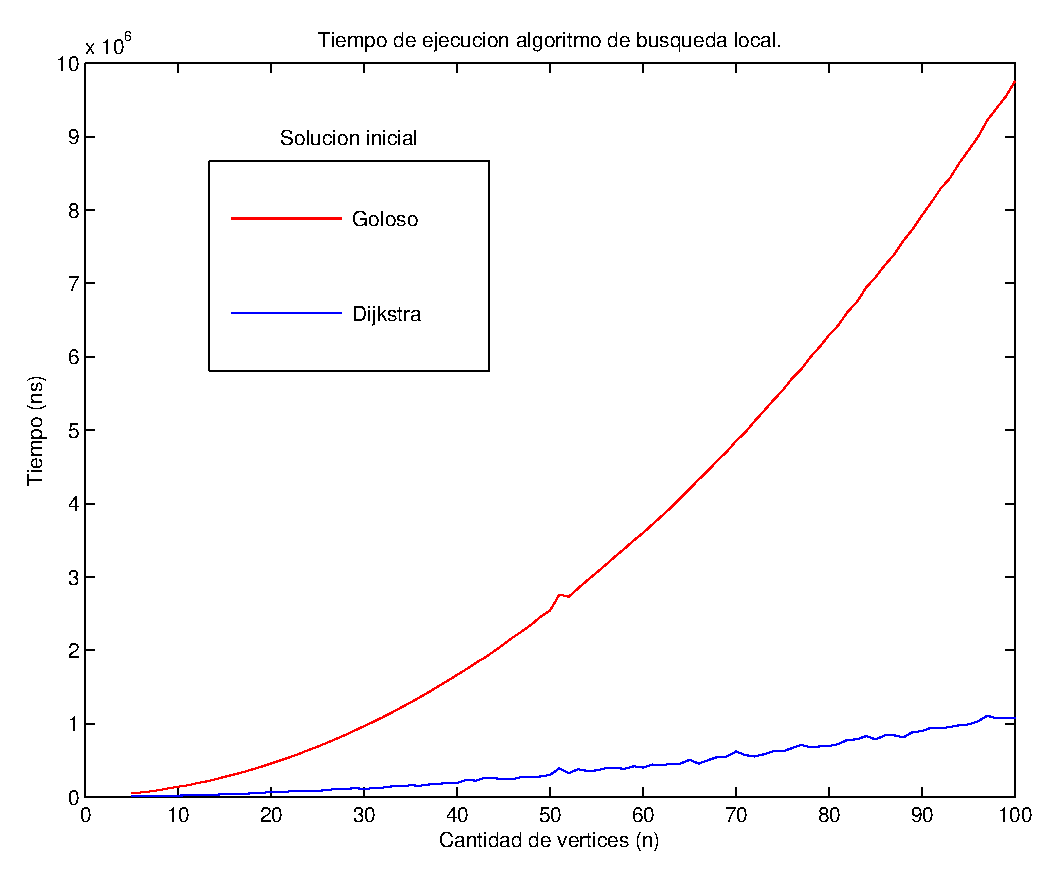
\includegraphics[width=\linewidth]{graficos/busq_local_tiempo.eps}
    \caption{Tiempo ejecución búsqueda local}\label{fig:busq-local-tiempo}
  \end{minipage}
  \hfill
  \begin{minipage}{0.5\linewidth}
    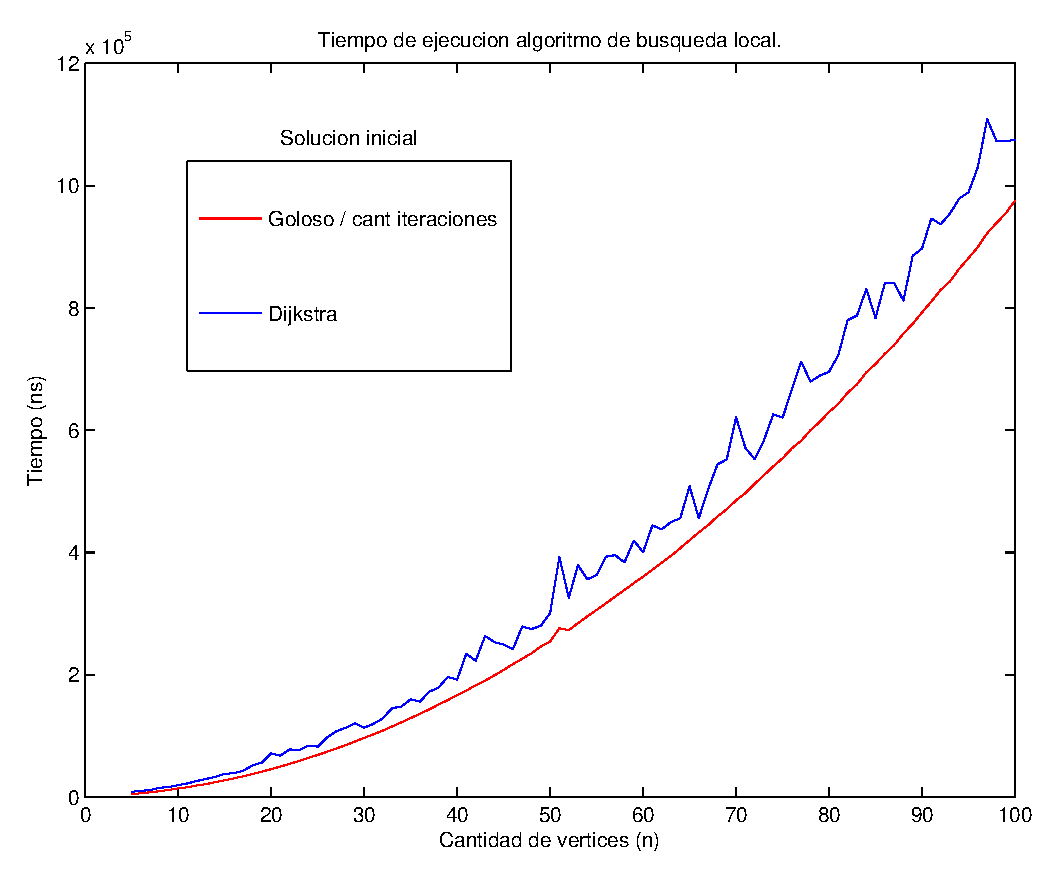
\includegraphics[width=\linewidth]{graficos/busq_local_tiempo_divido10.eps}
    \caption{Idem divido 10}\label{fig:busq-local-tiempo-div10}
  \end{minipage}
\end{figure}

Como podemos observar en el gráfico \ref{fig:busq-local-tiempo} el algoritmo de búsqueda local utilizando nuestro algoritmo goloso tiene un tiempo de ejecución mayor al que utiliza el algoritmo de Dijkstra. Esto se debe a que lo que medimos es el tiempo en correr primero los algoritmos que generan las soluciones iniciales y luego correr el algoritmo de búsqueda local. Como ya sabemos nuestro algoritmo goloso corre el algoritmo de Dijkstra una cantidad de iteraciones prefijada. Resulta lógico pensar que un algoritmo que corre el algoritmo de Dijkstra muchas veces tendrá un tiempo de ejecución mayor al de un algoritmo que lo corre sólo una.

Por esto en el gráfico \ref{fig:busq-local-tiempo-div10} mostramos los mismos tiempos que en el otro gráfico pero dividimos el tiempo que tarda el algoritmo de búsqueda local que usa nuestro algoritmo goloso por \emph{cant iteraciones}. Con este gráfico, logramos ver que el tiempo de ejecución de ambos algoritmos de búsqueda es parecido cuando reducimos el factor de tiempo de ejecución del algoritmo nos da la solución inicial.